\documentclass[10pt,landscape]{article}
\usepackage{multicol}
\usepackage{calc}
\usepackage{ifthen}
\usepackage[landscape]{geometry}
\usepackage{verbatim}
\usepackage{graphicx}
\usepackage{color}
\usepackage[usenames,dvipsnames,svgnames,table]{xcolor}

\usepackage{hyperref}
\hypersetup{colorlinks=true}



% To make this come out properly in landscape mode, do one of the following
% 1.
%  pdflatex latexsheet.tex
%
% 2.
%  latex latexsheet.tex
%  dvips -P pdf  -t landscape latexsheet.dvi
%  ps2pdf latexsheet.ps


% If you're reading this, be prepared for confusion.  Making this was
% a learning experience for me, and it shows.  Much of the placement
% was hacked in; if you make it better, let me know...


% 2008-04
% Changed page margin code to use the geometry package. Also added code for
% conditional page margins, depending on paper size. Thanks to Uwe Ziegenhagen
% for the suggestions.

% 2006-08
% Made changes based on suggestions from Gene Cooperman. <gene at ccs.neu.edu>


% To Do:
% \listoffigures \listoftables
% \setcounter{secnumdepth}{0}


% This sets page margins to .5 inch if using letter paper, and to 1cm
% if using A4 paper. (This probably isn't strictly necessary.)
% If using another size paper, use default 1cm margins.
\ifthenelse{\lengthtest { \paperwidth = 11in}}
	{ \geometry{top=.5in,left=.5in,right=.5in,bottom=.5in} }
	{\ifthenelse{ \lengthtest{ \paperwidth = 297mm}}
		{\geometry{top=1cm,left=1cm,right=1cm,bottom=1cm} }
		{\geometry{top=1cm,left=1cm,right=1cm,bottom=1cm} }
	}

% Turn off header and footer
\pagestyle{empty}
 
% Redefine section commands to use less space
\makeatletter
\renewcommand{\section}{\@startsection{section}{1}{0mm}%
                                {-1ex plus -.5ex minus -.2ex}%
                                {0.5ex plus .2ex}%x
                                {\normalfont\large\bfseries}}
\renewcommand{\subsection}{\@startsection{subsection}{2}{0mm}%
                                {-1explus -.5ex minus -.2ex}%
                                {0.5ex plus .2ex}%
                                {\normalfont\normalsize\bfseries}}
\renewcommand{\subsubsection}{\@startsection{subsubsection}{3}{0mm}%
                                {-1ex plus -.5ex minus -.2ex}%
                                {1ex plus .2ex}%
                                {\normalfont\small\bfseries}}
\makeatother



% Don't print section numbers
\setcounter{secnumdepth}{0}


\setlength{\parindent}{0pt}
\setlength{\parskip}{0pt plus 0.5ex}


% -----------------------------------------------------------------------

\begin{document}

\raggedright
\footnotesize
\begin{multicols}{3}


% multicol parameters
% These lengths are set only within the two main columns
%\setlength{\columnseprule}{0.25pt}
\setlength{\premulticols}{1pt}
\setlength{\postmulticols}{1pt}
\setlength{\multicolsep}{1pt}
\setlength{\columnsep}{2pt}

\begin{center}
     \Large{\textbf{Vim Cheat Sheet}} \\
\end{center}

\subsection{Start editing...}
\begin{tabular}{@{}ll@{}}
\verb!i!       & At the cursor \\
\verb!I!       & At the first non-whitespace of the line \\
\verb!a!       & After the cursor \\
\verb!A!       & After the last character of this line \\
\verb!o!       & New line after this one\\
\verb!O!       & New line before this one\\
\end{tabular}


\subsection{Copy, Paste, Delete}
\begin{tabular}{@{}ll@{}}
\verb!dd!      & Delete this line. \\
\verb!d10d!    & Delete 10 lines. \\
\verb!y3w!     & Copy 3 words. \\
\verb!pp!      & Paste deleted or copied text. \\
\end{tabular}

\subsection{Search and Replace}
\begin{tabular}{@{}ll@{}}
\verb!:%s/old/new/!          & Replace \verb!old! with \verb!new! globally\\
\verb!:%s/old/new/c!         & Ask for every match\\
\end{tabular}

\subsection{Undo and Redo}
\begin{tabular}{@{}ll@{}}
\verb!u!          & Undo\\
\end{tabular}

\subsection{Syntax Highlighting}
\begin{tabular}{@{}ll@{}}
\verb!:syntax {on|off}!      & Toggle syntax highlighting \\
\verb!:set bg={dark|light}!  & Adjust highlighting brightness \\
\end{tabular}



\rule{0.3\linewidth}{0.25pt}
\scriptsize

\includegraphics[width=10em]{by_nc_sa.eps}

This work is licensed under a \href{http://creativecommons.org/licenses/by-nc-sa/3.0/}{Creative Commons Attribution-NonCommercial-ShareAlike 3.0 Unported License}.

\copyright\ 2012 \href{http://matan.name}{Adam Matan}

Based on a \href{http://www.stdout.org/~winston/latex/}{\LaTeX\ template by Winston Chang}

\end{multicols}
\end{document}
